\section{Results}\label{sec:results}

We report each scenario's endpoint by model, prompt and harness, then the human calibration of the readout and the
pattern across scenarios. Figure~\ref{fig:results} gives the three
endpoints side by side. The 95\% intervals resample cases, retaining all
models, arms, prompts and witnesses within each case, and McNemar tests
are used only for single-model comparisons with one binary pair per paper.

\subsection{OpenReview: sensitivity to the review package}\label{sec:or-v2}\label{sec:or}

\begin{figure}[t]
\centering
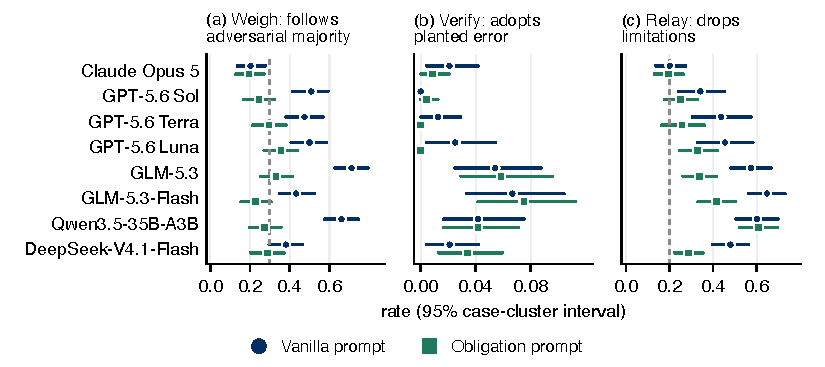
\includegraphics[width=\linewidth]{figures/fig_results_overview.pdf}
\caption{The three endpoints of \S\ref{sec:design}, eight models, two prompts. Each point is a
rate with its case-cluster 95\% interval. (a) OpenReview, majority following in the
adversarial arm: the program chair follows a generic 3:1 majority away
from the paper's real outcome. (b) Court, error adoption: the ruling repeats the planted
procedural-fact error as fact. (c) Parliament, limitation loss: a cited headline claim is
reproduced without either limitation its witness attached. Model order is
fixed across panels.}
\label{fig:results}
\end{figure}

\paragraph{Constructed adversarial votes.}\label{sec:or-v3}
With paper and rebuttal held fixed and the review package reversed
(\S\ref{sec:scenarios}), every model has more shifts toward than against
the new majority. Across 1{,}878 paired decisions of the eight paper
models, 621 decisions that matched the reference under control reviews
followed the generic majority away from it under adversarial reviews,
against 5 the other way (Table~\ref{tab:or-v3}). Under Vanilla, pooled
majority following is $0.48$ ($457$ of $944$, case-cluster CI $[0.43,
0.54]$), and Obligation lowers it to $0.28$. The 118 papers have
recorded historical decisions, 58 accepted with a mean score of at least
$6.5$ and 60 rejected with at most $4.5$; their real outcome is a
reference direction, not a gold standard of quality. Control-arm
agreement is at least $0.96$ under Vanilla, and the program chair's
decision matches the area chair's recommendation in $933$ of $944$
adversarial episodes under Vanilla and $891$ of $939$ under Obligation,
with Qwen3.5-35B-A3B accounting for $28$ of the $48$ Obligation
disagreements. Majority following thus originates with the area chair
and passes through the program chair.
\rev{That the second tier rarely overrides the first is itself a finding:
what the area chair does with the majority reaches the final decision
almost unchanged, even when the program chair is told to override vote
tallies.}

\begin{table}[t]\centering\small\setlength{\tabcolsep}{3.5pt}
\caption{Constructed votes: 118 papers, eight models. Ctrl and Adv give agreement with the majority in the control and adversarial review packages. Intervals are case-cluster 95\% intervals. Bold: lowest Adv within each prompt. Shift counts reference-consistent control decisions that follow the opposing majority under adversarial reviews / the reverse. Acc/Rej gives adversarial following for historically accepted/rejected papers, pooling prompts. Historical outcomes are reference labels.}
\label{tab:or-v3}
\resizebox{\linewidth}{!}{\begin{tabular}{l ccc ccc c}\toprule & \multicolumn{3}{c}{Vanilla} & \multicolumn{3}{c}{Obligation} & \\\cmidrule(lr){2-4}\cmidrule(lr){5-7}
Model & Ctrl & Adv [95\% CI] & Shift / reverse & Ctrl & Adv [95\% CI] & Shift / reverse & Acc / Rej \\\midrule
Claude Opus 5 & 0.98 & \textbf{0.20 [0.14, 0.28]} & 22 / 0 & 0.92 & \textbf{0.19 [0.13, 0.27]} & 15 / 1 & 0.20 / 0.20 \\
GPT-5.6 Sol & 0.99 & 0.51 [0.42, 0.59] & 59 / 0 & 0.84 & 0.25 [0.17, 0.32] & 11 / 1 & 0.50 / 0.26 \\
GPT-5.6 Terra & 0.97 & 0.47 [0.38, 0.57] & 53 / 0 & 0.87 & 0.30 [0.21, 0.38] & 20 / 0 & 0.54 / 0.23 \\
GPT-5.6 Luna & 0.97 & 0.50 [0.41, 0.58] & 56 / 0 & 0.83 & 0.36 [0.27, 0.44] & 22 / 0 & 0.72 / 0.15 \\
GLM-5.3 & 1.00 & 0.71 [0.63, 0.80] & 84 / 0 & 1.00 & 0.33 [0.25, 0.42] & 39 / 0 & 0.42 / 0.62 \\
GLM-5.3-Flash & 1.00 & 0.43 [0.35, 0.53] & 51 / 0 & 0.95 & 0.23 [0.15, 0.31] & 20 / 0 & 0.16 / 0.50 \\
Qwen3.5-35B-A3B & 0.99 & 0.66 [0.58, 0.75] & 75 / 0 & 1.00 & 0.27 [0.20, 0.36] & 32 / 0 & 0.46 / 0.48 \\
DeepSeek-V4.1-Flash & 0.97 & 0.38 [0.30, 0.47] & 41 / 0 & 0.86 & 0.29 [0.20, 0.37] & 21 / 3 & 0.37 / 0.30 \\
\midrule
Pooled & 0.99 & 0.48 [0.43, 0.54] & 441 / 0 & 0.91 & 0.28 [0.23, 0.33] & 180 / 5 & 0.42 / 0.34 \\
\bottomrule\end{tabular}}\end{table}


Under Vanilla, chairs follow a generic 3/3/2 majority on an accepted
paper ($0.50$, $[0.43, 0.58]$) about as often as a generic 7/7/8 majority
on a rejected one ($0.46$, $[0.38, 0.55]$). The Obligation gain is not a
uniform shift: of $939$ paper--model pairs with valid adversarial
decisions under both prompts, $234$ follow the generic majority under
both, $222$ only under Vanilla, $26$ only under Obligation and $457$ under
neither.

\rev{\paragraph{What drives majority following.} Following a majority is
not by itself a failure, and the adversarial arm changes scores, stance and
specificity together. Four controls separate these
(Table~\ref{tab:or-controls}; per model in
Table~\ref{tab:or-controls-models}). An agent that sees only the paper
would follow the adversarial majority at its own paper-only disagreement
with the historical decision; under Vanilla, pooled following exceeds this
reference by $0.17$ ($[0.13, 0.21]$), from $0.00$ for Claude Opus~5 to
$0.47$ for GLM-5.3, and under Obligation the excess disappears. Removing
every numeric score barely changes following, so the pull comes from the
stance of the review texts. With two specific against two generic reviews,
agents follow the specific side above the paper-only reference whichever
side it argues, and following rises with the size of the majority but not
with the dissenter's position. Agents thus favour the more specific side when
counts are equal, but a growing majority increasingly overrides their own
reading of the paper. Reviews new to these controls passed mechanical checks
(stated score, matched length) but not the blind rating.}

\begin{table}[t]\centering\small\setlength{\tabcolsep}{4pt}
\caption{\rev{Controls for the review package (OpenReview, constructed votes; 118 papers and eight models unless noted). Rates of program-chair decisions. Paper only: the agent sees the paper but no reviews or rebuttal; an agent that ignores the reviews would follow the adversarial majority at the rate of its paper-only disagreement with the historical decision (reference). Excess: same paper, model and prompt, adversarial following minus that reference. No scores: every numeric score removed from reviews and responses, change against the original adversarial arm. 2:2: two specific reviews against two generic reviews on the other side, with the specific side for (SP) or against (SM) the historical decision; parentheses give the paper-only reference. Ratio and order: 30 papers, four models.}}
\label{tab:or-controls}
\begin{tabular}{l l cc}\toprule
Design & Quantity & Vanilla & Obligation \\ \midrule
Adversarial 3:1 & follows majority & 0.48 & 0.28 \\
Paper only & reference & 0.31 & 0.34 \\
 & excess over reference & $+$0.17 & $-$0.06 \\
No scores & change in following & $-$0.03 & $-$0.01 \\
2:2, SP & follows specific side & 0.86 (0.69) & 0.83 (0.66) \\
2:2, SM & follows specific side & 0.51 (0.31) & 0.48 (0.34) \\ \midrule
Ratio 2:1 / 3:1 / 4:1 & follows majority & 0.28 / 0.53 / 0.62 & 0.24 / 0.27 / 0.37 \\
3:1, dissenter first & follows majority & 0.45 & 0.27 \\
\bottomrule\end{tabular}\end{table}


\paragraph{Argument quality against real votes.}
The votes had to be constructed because decisions rarely moved when
only argument quality was swapped under the real 3:1 score split of 119
ICLR submissions. Of $711$ valid Vanilla pairs, $691$ were identical across arms
($12$ versus $8$ flips toward the minority and majority); Obligation gave
$49$ against $22$ (Table~\ref{tab:app-contrasts}).
The chairs' agreement with the
historical decision across arms and prompts ($0.76$--$0.78$) tracked that
of the majority they were given ($0.78$), and because that majority usually
matches the reference, this design cannot tell whether the split
or the paper drove it. \rev{This design uses the original paper text, of
which 25 of the 119 are camera-ready versions; the arm contrast holds that
text fixed, but agreement with the historical decision is not interpreted.}

\subsection{Court: the planted error rarely reaches the ruling}
\label{sec:court}
Judges adopted the planted error in $111$ of $3{,}832$ rulings ($2.9\%$,
case-cluster CI $[2.0, 3.9]$), well below the $0.20$ we had set in
advance as the threshold for a substantive failure
(Figure~\ref{fig:results}b; Table~\ref{tab:court},
Appendix~\ref{app:extra}). GLM-5.3, GLM-5.3-Flash and Qwen3.5-35B-A3B
account for $81$ of the $111$. The low rate shows the error rarely reaches
the ruling when the correct record is available, not that the judge
checked the record rather than recalled the case.

The Obligation prompt changes not whether the error is adopted but
whether it is confronted. Pooled over the eight models, the correction
rate rises from $0.09$ under Vanilla to $0.25$ under Obligation, a
paired increase of $0.16$ with case-cluster interval $[0.14, 0.18]$.
Under Vanilla only Claude Opus~5 routinely names counsel's
error and rejects it ($0.53$); with the obligation stated, corrections
rise for Opus to $0.84$, for Sol from $0.01$ to $0.28$ and for GLM-5.3
from $0.03$ to $0.24$, while Luna and Qwen do not move. DeepSeek-V4.1-Flash
follows the same pattern from a higher base, $0.10$ to $0.47$.

\subsection{Parliament: witness limitations are dropped, and not evenly}
\label{sec:parliament}
\begin{table}[tb]\centering\small\setlength{\tabcolsep}{3.5pt}
\caption{Parliament: 120 inquiries, eight models, 120 reports per model/prompt. Aligned/opposed (a/o) refer to the stored historical reference. Cited is the fraction of reports citing each claim; QL is the fraction of cited claims losing both limitations, with case-cluster 95\% intervals, followed by a/o rates. Bold: lowest QL within each prompt.}
\label{tab:parliament}
\resizebox{\linewidth}{!}{\begin{tabular}{l ccc ccc}\toprule & \multicolumn{3}{c}{Vanilla} & \multicolumn{3}{c}{Obligation} \\\cmidrule(lr){2-4}\cmidrule(lr){5-7}
Model & Cited a / o & QL [95\% CI] & QL a / o & Cited a / o & QL [95\% CI] & QL a / o \\\midrule
Claude Opus 5 & 0.68 / 0.61 & \textbf{0.20 [0.14, 0.28]} & 0.26 / 0.14 & 0.65 / 0.71 & \textbf{0.20 [0.13, 0.26]} & 0.21 / 0.19 \\
GPT-5.6 Sol & 0.34 / 0.32 & 0.34 [0.24, 0.45] & 0.32 / 0.37 & 0.50 / 0.49 & 0.25 [0.18, 0.33] & 0.27 / 0.24 \\
GPT-5.6 Terra & 0.34 / 0.19 & 0.44 [0.30, 0.57] & 0.49 / 0.35 & 0.44 / 0.33 & 0.26 [0.16, 0.36] & 0.26 / 0.25 \\
GPT-5.6 Luna & 0.29 / 0.26 & 0.45 [0.33, 0.58] & 0.49 / 0.42 & 0.46 / 0.40 & 0.33 [0.25, 0.42] & 0.36 / 0.29 \\
GLM-5.3 & 0.62 / 0.46 & 0.57 [0.48, 0.67] & 0.64 / 0.49 & 0.65 / 0.56 & 0.34 [0.26, 0.41] & 0.40 / 0.27 \\
GLM-5.3-Flash & 0.62 / 0.54 & 0.65 [0.56, 0.73] & 0.64 / 0.66 & 0.57 / 0.57 & 0.42 [0.33, 0.50] & 0.41 / 0.42 \\
Qwen3.5-35B-A3B & 0.48 / 0.33 & 0.60 [0.51, 0.70] & 0.59 / 0.62 & 0.52 / 0.48 & 0.61 [0.52, 0.69] & 0.60 / 0.62 \\
DeepSeek-V4.1-Flash & 0.65 / 0.58 & 0.48 [0.40, 0.56] & 0.50 / 0.46 & 0.74 / 0.71 & 0.29 [0.22, 0.35] & 0.34 / 0.24 \\
\midrule
Pooled & 0.50 / 0.41 & 0.47 [0.41, 0.53] & 0.49 / 0.44 & 0.57 / 0.53 & 0.33 [0.28, 0.38] & 0.35 / 0.31 \\
\bottomrule\end{tabular}}\end{table}


Pooled over the eight evaluated models and both conditions, $759$ of
$1{,}931$ cited headline claims ($0.39$, case-cluster CI $[0.35, 0.44]$)
were reproduced without the limitations the witness had placed on them,
twice the $0.20$ we had set in advance (Table~\ref{tab:parliament}).
Claude Opus~5 alone sits at the threshold. Under Vanilla, a sample-size
caveat or scope restriction in the witness's own sentence becomes an
unconditional finding in the report in one citation in five for Opus, one
in three to one in two for the GPT-5.6 variants and DeepSeek, and six in
ten for GLM and Qwen.

Under Vanilla, $251$ reports cite only the aligned witness and $164$
only the opposed witness, where alignment refers to the stored
historical reference, not a randomized condition or the agent's own
conclusion. The citation-rate difference is $0.091$ with case-cluster
interval $[0.016,0.164]$, while the conditional-loss difference ($0.49$
versus $0.44$, $[-0.035,0.152]$) is not directional.

Obligation reduces pooled limitation loss by $0.136$ ($[0.095,0.179]$
reduction). Individual intervals exclude zero for GLM-5.3, GLM-5.3-Flash,
Terra and DeepSeek, and Qwen's point estimate rises. Citation
coverage also rises, from $0.46$ to $0.55$, so part of the pooled change
could come from citing different claims. Pairing the $1{,}920$ witness
slots across prompts separates the two:
among $723$ claims cited under both prompts, loss falls from $0.46$ to
$0.33$, with limitations restored on $139$ claims and newly dropped on
$51$, while Obligation adds $331$ citations and removes $154$.

\subsection{Human assessment of the readout}\label{sec:human}

Three annotators, blind to model, prompt and machine label, labeled a
stratified sample of $100$ Court rulings, $100$ Parliament reports ($200$
witness slots) and $30$ generated reviews
(Appendix~\ref{app:human-calibration}). We compare the readout
with their majority label. The semantic layer agrees with it at
$\kappa=0.63$ in Court and $0.68$ in Parliament ($0.75$ and $0.79$ where
all three agree); pattern rules alone match it on $3$ of $84$ Court
rulings. Two rates need qualification. In Court, the majority confirms
$5$ of the $15$ semantic adoptions in the sample and adds none, so
disagreement runs toward over-labeling adoption. In Parliament, loss among cited claims is
$0.47$ by machine and by majority but $0.14$--$0.85$ across annotators,
so it compares models under one reading of the label, not as an
absolute rate. \rev{Reweighted by each reader's labels
(Table~\ref{tab:label-sensitivity}), Court adoption stays low and both
Obligation effects hold under the majority and two of three annotators.}

\subsection{Across scenarios}\label{sec:cross}

Failure rates differ by more than an
order of magnitude and model orderings differ across scenarios, so we
report RI together with its components
(Table~\ref{tab:ri}), each measuring a different obligation.

\begin{table}[t]\centering\small\setlength{\tabcolsep}{4pt}
\caption{Role integrity (RI), the unweighted mean of the three kept-obligation fractions, one minus each scenario's adverse rate, ordered by Vanilla RI. Bold: highest value in each column within each prompt. Intervals are in Table~\ref{tab:ri-ci}. Index: rank among these eight models on the Artificial Analysis Intelligence Index \citep{artificialanalysis2026index}, highest listed entry per model; tied scores share a rank. ${}^\dag$Entry marked estimated by the index.}
\label{tab:ri}
\begin{tabular}{l cccc cccc c}\toprule
 & \multicolumn{4}{c}{Vanilla} & \multicolumn{4}{c}{Obligation} & \\ \cmidrule(lr){2-5}\cmidrule(lr){6-9}
Model & Weigh & Verify & Relay & RI & Weigh & Verify & Relay & RI & Index \\ \midrule
Claude Opus 5 & \textbf{0.80} & 0.98 & \textbf{0.80} & \textbf{0.86} & \textbf{0.81} & 0.99 & \textbf{0.80} & \textbf{0.87} & 1 \\
GPT-5.6 Sol & 0.49 & \textbf{1.00} & 0.66 & 0.72 & 0.75 & \textbf{1.00} & 0.75 & 0.83 & 2 \\
DeepSeek-V4.1-Flash & 0.62 & 0.98 & 0.52 & 0.71 & 0.71 & 0.97 & 0.71 & 0.80 & 6 \\
GPT-5.6 Terra & 0.53 & 0.99 & 0.56 & 0.69 & 0.70 & \textbf{1.00} & 0.74 & 0.82 & 4 \\
GPT-5.6 Luna & 0.50 & 0.97 & 0.55 & 0.67 & 0.64 & \textbf{1.00} & 0.67 & 0.77 & 7 \\
GLM-5.3-Flash & 0.57 & 0.93 & 0.35 & 0.62 & 0.77 & 0.93 & 0.58 & 0.76 & 4 \\
Qwen3.5-35B-A3B & 0.34 & 0.96 & 0.40 & 0.57 & 0.73 & 0.96 & 0.39 & 0.69 & 8\dag \\
GLM-5.3 & 0.29 & 0.95 & 0.43 & 0.55 & 0.67 & 0.94 & 0.66 & 0.76 & 3 \\
\bottomrule\end{tabular}
\end{table}


Agents read what they were given. The median episode opens every file
in the case directory, 5 in Court, 11 in Parliament and 12 or 13 in
OpenReview, and median wall time per role runs from 10 seconds for the
GPT-5.6 Luna program chair in OpenReview to 240 seconds for Claude Opus~5
in Parliament.

The spread in RI comes almost entirely from weighing and relaying, since
every model keeps the verification obligation on at least $0.92$ of
rulings, and orderings differ across components: Opus leads on weighing
and relaying but not on verification. Obligation prompts raise RI for every
model.

General capability does not order these results. On a third-party
capability index (Table~\ref{tab:ri}, Appendix~\ref{app:extra}), Claude
Opus~5 is first on both, but the order below it diverges: GLM-5.3 is
third on the index and last on RI under Vanilla, GLM-5.3-Flash ties for
fourth and is sixth, DeepSeek-V4.1-Flash is sixth on the index and third on
RI, and Qwen3.5-35B-A3B, last on the index, is seventh.

\subsection{The same model under a different harness}\label{sec:harness}

Every result above runs the senior role in one harness. To see how much
of a model's RI belongs to the harness rather than the model, we reran two
models on a hard subset under a second harness each.
The subset is the 20 cases per scenario with the highest failure rate
among the six models other than the two rerun models. Sol ran
under \texttt{pi} and under the Codex CLI \citep{openai2026codexcli};
DeepSeek-V4.1-Flash ran under \texttt{pi} and under DeepSeek's own
harness (\texttt{dsh}) \citep{deepseek2026harness}.

\begin{table}[h]\centering\small\setlength{\tabcolsep}{4pt}
\caption{Harness variance on the hard subset: 20 cases per scenario, each model run under two harnesses with the same prompts, cases and readout. Cells give the kept-obligation fraction with the adverse count over its denominator (majority-following decisions over valid adversarial-arm decisions; adopted errors over rulings; unqualified citations over cited claims). Intervals are case-cluster 95\% intervals; Vanilla and Obligation come from different episodes.}
\label{tab:harness}
\begin{tabular}{l l ccc c l}\toprule
Model, harness & Prompt & Weigh & Verify & Relay & RI & 95\% CI \\ \midrule
GPT-5.6 Sol, \texttt{pi} & Vanilla & 0.05 (19/20) & 1.00 (0/40) & 0.27 (11/15) & 0.44 & [0.35, 0.54] \\
GPT-5.6 Sol, \texttt{pi} & Obligation & 0.50 (10/20) & 1.00 (0/40) & 0.48 (12/23) & 0.66 & [0.55, 0.76] \\
\addlinespace[2pt]
GPT-5.6 Sol, \texttt{codex} & Vanilla & 0.25 (15/20) & 1.00 (0/40) & 0.15 (11/13) & 0.47 & [0.37, 0.58] \\
GPT-5.6 Sol, \texttt{codex} & Obligation & 0.60 (8/20) & 1.00 (0/40) & 0.29 (12/17) & 0.63 & [0.53, 0.74] \\
\addlinespace[2pt]
DeepSeek-V4.1-Flash, \texttt{pi} & Vanilla & 0.30 (14/20) & 0.90 (3/31) & 0.29 (15/21) & 0.50 & [0.41, 0.59] \\
DeepSeek-V4.1-Flash, \texttt{pi} & Obligation & 0.40 (12/20) & 0.88 (4/32) & 0.27 (19/26) & 0.51 & [0.42, 0.61] \\
\addlinespace[2pt]
DeepSeek-V4.1-Flash, \texttt{dsh} & Vanilla & 0.16 (16/19) & 0.78 (8/36) & 0.32 (17/25) & 0.42 & [0.33, 0.52] \\
DeepSeek-V4.1-Flash, \texttt{dsh} & Obligation & 0.45 (11/20) & 0.89 (4/36) & 0.69 (10/32) & 0.68 & [0.58, 0.77] \\
\bottomrule\end{tabular}\end{table}


For GPT-5.6 Sol the two harnesses trade components, Codex weighing
better and relaying worse, and RI changes by $+0.03$ under Vanilla and
$-0.03$ under Obligation, with case-cluster intervals $[-0.07, 0.12]$ and
$[-0.12, 0.08]$. For DeepSeek the harness matters under one prompt and
not the other: \texttt{dsh} is $0.08$ below \texttt{pi} under Vanilla
($[-0.20, 0.05]$) and $0.16$ above it under Obligation ($[0.07, 0.25]$),
almost all of it in relaying. The Obligation prompt itself raises RI by
$0.22$ and $0.16$ for Sol in the two harnesses and by $0.26$ for
DeepSeek in \texttt{dsh}, but by only $0.02$ ($[-0.06, 0.09]$) for
DeepSeek in \texttt{pi}. The rerun of Sol under the paper harness sits $0.08$ and $0.12$ above
its full-run episodes on the same 20 cases, more than the Sol harness
contrasts, so for Sol we cannot separate harness from run-to-run
variation. The hard subset was selected on the failures of
other models, so absolute values are not comparable to Table~\ref{tab:ri}.
